\documentclass{article}
%%%%%%%%%%%%%%% Declare Package: %%%%%%%%%%%%%
\usepackage{graphicx}% to insert graph
\usepackage{float}
\usepackage{tikz}
\usetikzlibrary{arrows, arrows.meta}
\usepackage[text=red]{callouts}%% annotation for figures
%%%%%%%%%%%%%% Title and author: %%%%%%%%%%%%%

%%%%%%%%%%%%%% Begin document: %%%%%%%%%%%%%%%
\begin{document}
%%%%%%%%%%%%%%% Custom commands: %%%%%%%%%%%%
\begin{figure}
    \centering
    \begin{annotate}{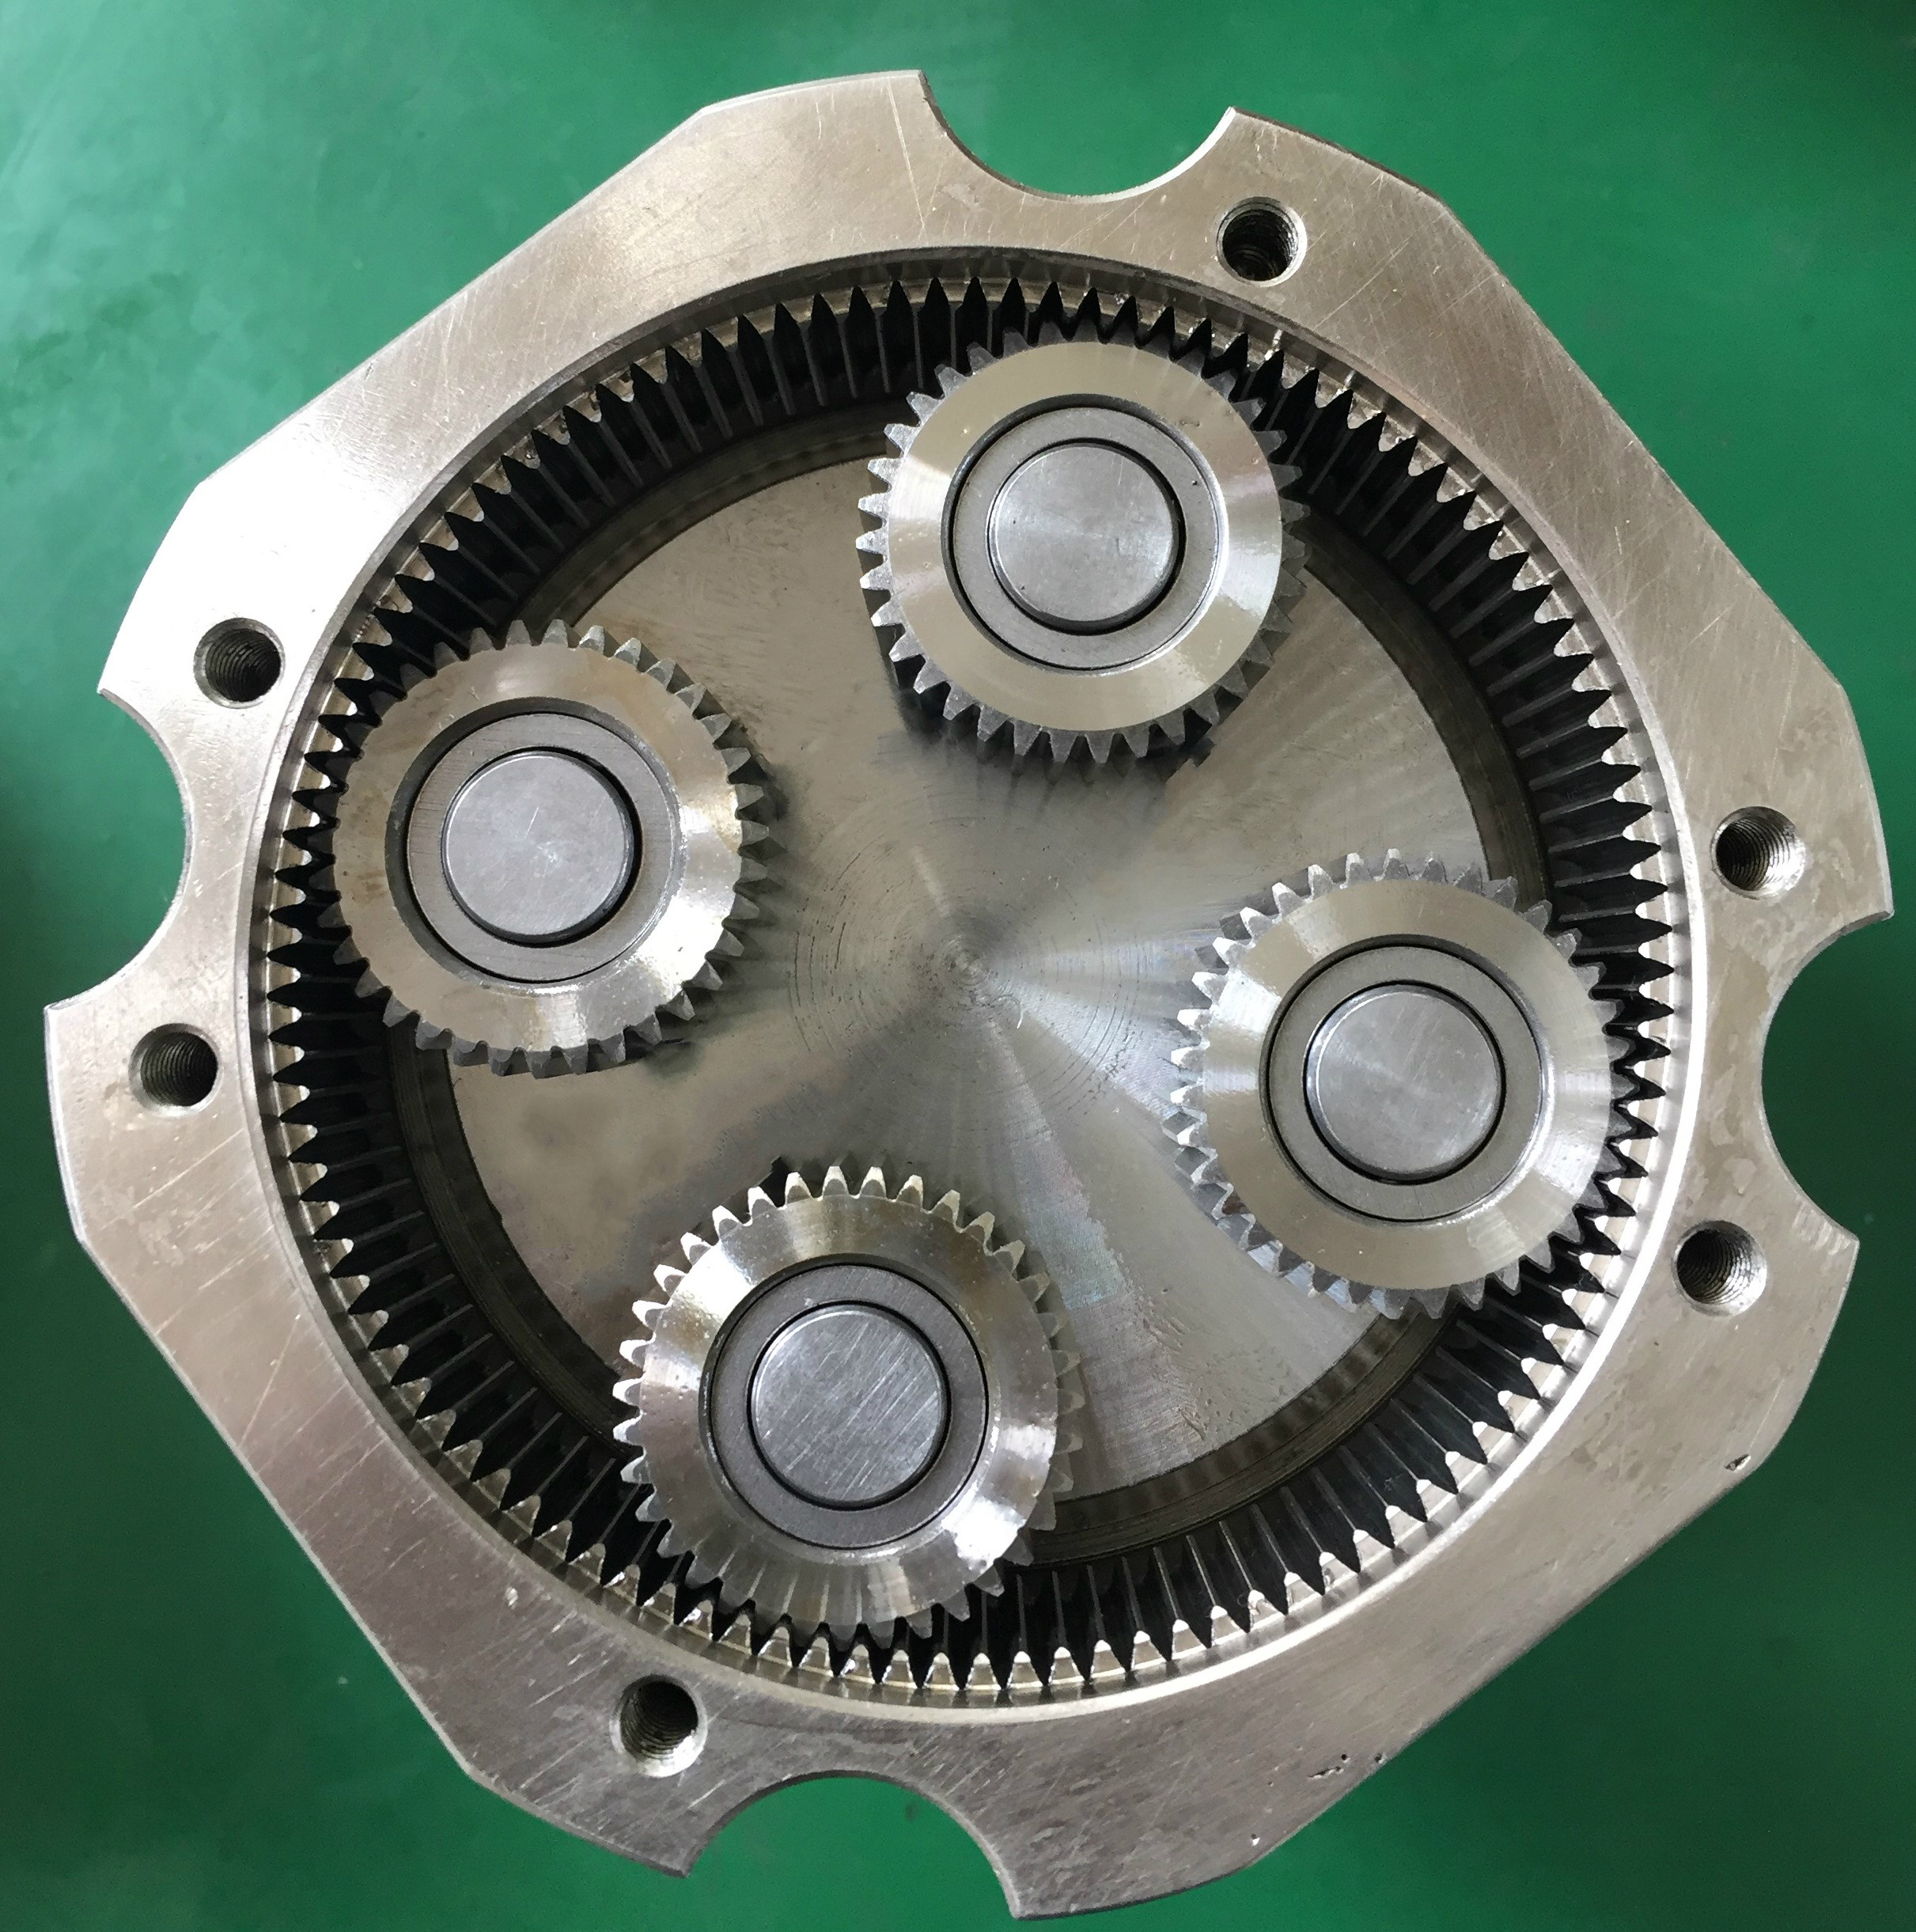
\includegraphics[width=0.5\textwidth]{exp_pinhole_error.jpg}}{1}
%\helpgrid[gray]
\draw [color=red]  (0,0) -- (-14:2);
\draw [color=red]  (0,0) -- (74:2);
\draw [color=red]  (0,0) -- (165:2);
\draw [color=red] (0,0) -- (-104:2);
\draw [-to,color=red] (-104:0.5) arc(-104:-195:0.5) (-195:0.5);
\draw [color=red,-to] (-104:0.5) -- (-103:0.5);
\note{-1,-0.5} {\angle$=90.1^\circ$}
    \end{annotate}

\end{figure}

\end{document}